\section{Lektion 30-01-2018}

\begin{enumerate}
	\item Course introduction
	\item Typical embedded system
	\item Number formats (fixed- and floating-point)
	\item Conversion between different number formats
	\item (Blackfin) DSP Architecture
	\item Software development flow
\end{enumerate}

\begin{mdframed}[style=exampledefault]
\begin{itemize}
	\item ESP Chapter 1.1 + 1.2
	\item ESP 5.1 + 5.2.1
	\item ESP Chapter 6.1.1 (only p.217-p.222) and 6.1.3 - 6.1.5
\end{itemize}
\end{mdframed}

\subsection{Typical embedded system}

\begin{itemize}
	\item \textbf{Dedicated functions:} Embedded systems usaully execute a specific task repeatedly. 
	\item \textbf{Tight constraints:} There are many constraints in designing an embedded system, such as; cost, processing speed, size, power consuption. 
	\item \textbf{Reactive and real-time performance:} Many embedded systems must continously react to changes of the system's input.
\end{itemize}

\subsection{Number formats (fixed- and floating-point)}
\begin{itemize}
	\item Fixed‐point
	\item Floating‐point
	\item Block floating‐point
\end{itemize}

\subsubsection{Fixed-point}

\begin{itemize}
	\item  Binary data format - signed and unsigned
	\begin{itemize}
		\item  The 2's complement format is	the most popular signed number in DSP processors.
		\item Most DSP processors support both integer and fractional data formats.
		\begin{itemize}
			\item  In an integer format, the radix point is located to the right of the least
			significant bit (LSB).
			\item In a fractional number format, the radix point is located within the binary number. 
			\begin{itemize}
				\item The number to the right	of the radix point assumes a fractional binary bit, with a weighting of $2^{-p}$ where the lowest fractional increment is $2^{−4}$ (or $0.0625$) in \ref{fig:1}.
				\item For the number to the left of the radix point, the weighting increases from $2^q$. The weighting of the MSB (or sign bit) depends on whether the number is signed or unsigned. 
			\end{itemize}
			\item (N.M) notation
			\begin{itemize}
				\item  N is the number of bits to the left of the radix point (integer part).
				\item M is the number of bits to the right of the radix point (fractional part). 
				\item The symbol \textit{"."} represents the radix point. 
				\item Total number of bits in the data word is B = N + M. 
			\end{itemize}
		\end{itemize}
	\end{itemize}
\end{itemize}

\begin{figure} [H]
	\centering
	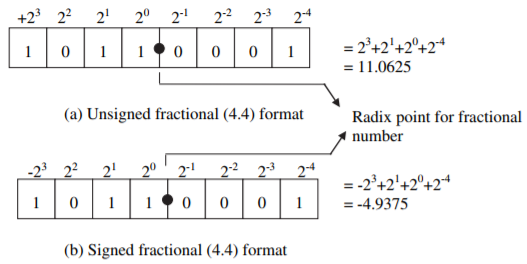
\includegraphics[width=0.85\linewidth]{graphics/1.png}
	\caption{Example of 8-bit binary data formats for a fractional number.}
	\label{fig:1}
\end{figure}

\begin{itemize}
	\item Dynamic Ranges and Precisions
	\begin{itemize}
		\item The maximum positive number in (1.15) format is $1 − 2^{−15} (= 0.999969482421875)$ (0x7FFF).
		\item The minimum negative number in (1.15) format is $−1$ (0x8000). 
		\item The 1.15 format has a \textbf{dynamic range} of $[+0.999969482421875$ to $−1]$
		\begin{itemize}
			\item Numbers exceeding this range cannot be represented in 1.15 format. 
		\end{itemize} 
		\item The smallest increment (or precision) within the (1.15) format is $2^{−15}$.
	\end{itemize}
	\item Scaling Factors
	\begin{itemize}
		\item A number in (N.M) format cannot be represented in the programs because most compilers and assemblers only recognize numbers in integer or (16.0) format. 
		\begin{itemize}
			\item Convert the fractional number in (N.M) format into its integer equivalent.
			\item Its radix point must be accounted for by the programmers.
			\begin{itemize}
				\item To convert a number $0.6$ in (1.15) format to its integer representation,
				multiply it by $2^{15}$ (or $32\,768$) and round the product to its nearest integer to
				become $19\,661$ (0x4CCD).
			\end{itemize}
		\end{itemize}
	\end{itemize}
\end{itemize}

 In table \ref{fig:2} all 16 possible (N.M) formats for 16-bit numbers. Different formats give different dynamic ranges and precisions. There is a trade-off between the dynamic range and precision.
 \begin{itemize}
 	\item As the dynamic range increases, precision becomes	coarser.
 \end{itemize}
 
 \begin{figure} [H]
 	\centering
 	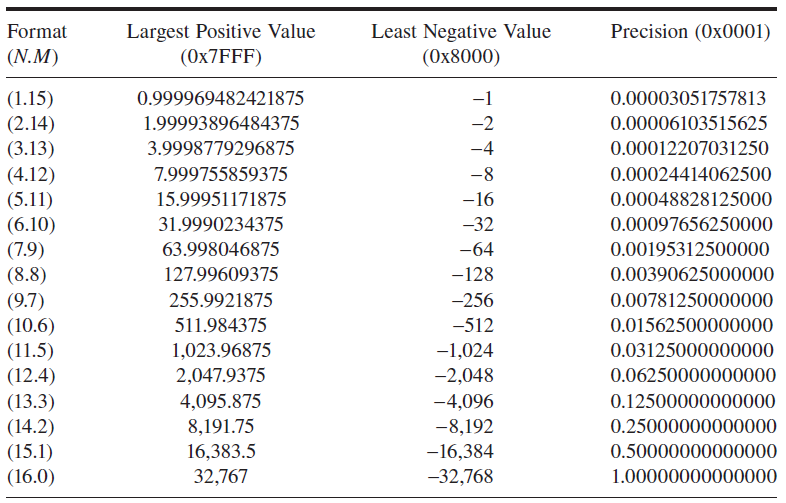
\includegraphics[width=\linewidth]{graphics/2.png}
 	\caption{Dynamic ranges and precisions of 16-bit numbers using different formats.}
 	\label{fig:2}
 \end{figure}



\subsection{Conversion between different number formats}
\subsubsection{Fixed-Point Data Types}
The Blackfin C compiler supports eight scalar data types and two fractional data types.

 \begin{figure} [H]
	\centering
	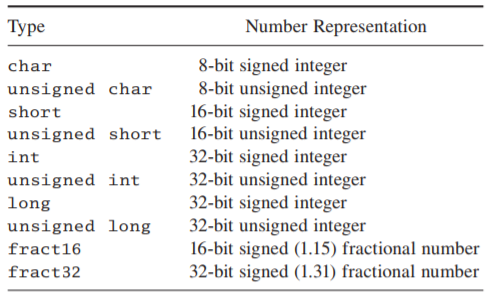
\includegraphics[width=0.85\linewidth]{graphics/3.png}
	\caption{Fixed-Point Data Types.}
	\label{fig:3}
\end{figure}

\subsection{(Blackfin) DSP Architecture}

\subsection{Software development flow}